\documentclass{article}
\usepackage[margin=0.7in]{geometry}
\usepackage{fancyhdr}
\pagestyle{fancy}
\fancyhf{}
\rhead{Sam Robbins}
\rfoot{Page \thepage}


\usepackage{beamerarticle}
\usepackage{enumerate}
\usepackage{xcolor}
\usepackage{tikz}
\usepackage{fancyvrb}
\usepackage{hyperref}
\usepackage{minted}
\definecolor{links}{HTML}{2A1B81}
\hypersetup{colorlinks,linkcolor=,urlcolor=blue}
\usetikzlibrary{shapes.misc}
\usetikzlibrary{shapes.geometric, arrows, positioning}

\title{Systems Programming --- Lecture 1:\\
Introduction to C Programming}
\author{Dr Konrad Dabrowski\\
\href{mailto://konrad.dabrowski@durham.ac.uk}{konrad.dabrowski@durham.ac.uk}
}
\date{E103 Christopherson Building}

\begin{document}

\maketitle




\section{Key topics for sub-module}
\begin{itemize}
\item Syntax and semantics of the C programming language
\item Memory access and management
\item Design of large programs in non-object-oriented language
\item Unix/Linux shell programming
\item A dash of C++
\end{itemize}



\section{Course details}
\begin{itemize}
\item Intro, HelloWorld, Compiling, Pre-processor
\item Control flow and functions
\item Data types, structs and unions
\item Memory access using pointers
\item Dynamic memory management
\item Scope of variables and recursive functions
\item Large programs and external libraries
\item Debugging
\item UNIX/Linux and C
\item C++
\end{itemize}

First practical: Week 3\\
Summative Assessment: Coursework (hand-out 7th February, hand-in 29th February)



\section{Resources and Books}

\begin{itemize}
\item The traditional text for C programming is
\emph{``The C Programming Language''}, Kernighan and Ritchie, Second Edition, Prentice Hall, ISBN 0-13-110362-8
(good reference book, although some aspects are a little dated. Exercise answers: \url{https://web.archive.org/web/*/http://www.trunix.org/programlama/c/kandr2/})

\item Based on the Kernighan and Ritchie book Steve Summit has a good set of free tutorial notes on C programming: \url{http://www.eskimo.com/~scs/cclass/}

\item An excellent and comprehensive modern book is: 
\emph{``C Programming A Modern Approach''}, K.N. King, Second Edition, ISBN 978-0-393-97950-3

\item See \url{https://stackoverflow.com/questions/562303/the-definitive-c-book-guide-and-list} for other book suggestions.
\end{itemize}



\section{Course Requirements}
\begin{itemize}
\item Some background assumed in programming
\item There are some references and comparisons to Java
\end{itemize}



\section{Standardisation of the C Language}
\begin{description}
\item[K\&R C]
Described in Kernighan and Ritchie, The C Programming Language (1978)
De facto standard
\item[C89/C90] ANSI standard X3.159-1989 (completed in 1988; formally approved in December 1989)\\
International standard ISO/IEC 9899:1990
\item[C99] International standard ISO/IEC 9899:1999 Incorporates changes from Amendment 1 (1995)
\item[C11] International standard ISO/IEC 9899:2011
\item[C18] ISO/IEC 9899:2018 -- the current standard for C
\item[C2x] Next version of the standard expected in 2021/2022
\end{description}



\section{C-based Languages}
\begin{description}
\item[C++] includes (almost) all the features of C, but adds classes and other features to support object-oriented programming
\item[Java] is based on C++ and therefore inherits many C features
%KD: Check next line
\item[Objective-C] is another OO extension for C, used in OSX/iOS development
\item[C\#] is a more recent language derived from   C++ and Java
\item[Perl] has adopted many of the features of C
\item + many others
\end{description}



\section{Why Choose C?}
\begin{center}
\scalebox{0.5}{\hspace*{-3cm}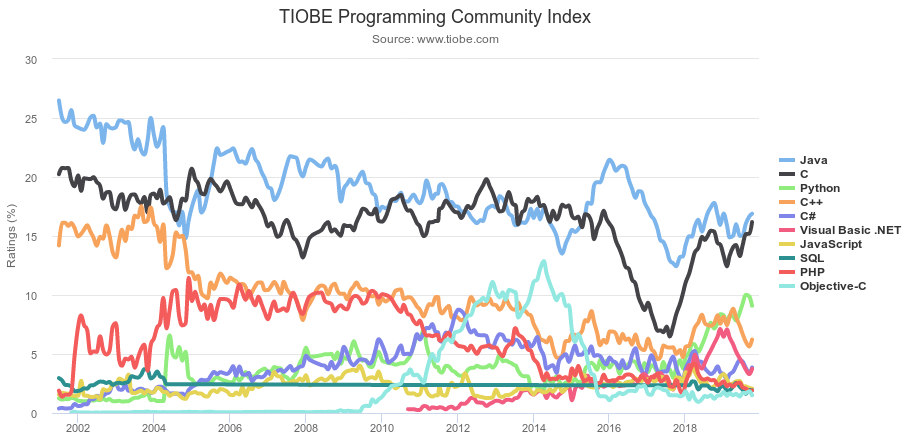
\includegraphics{tiobe.png}\hspace*{-3cm}}
\end{center}



\section{The C Language}
\begin{itemize}
\item Low-level -- close to assembly language
\item Small core language
\item Lots of well tested and freely available libraries
\item Compiled not interpreted (in principle)
\item Permissive -- dangerous -- no warnings
\end{itemize}



\section{A First Program}

\begin{minted}{c}
#include<stdio.h>
int main() 
{    
    printf("Hello, World!\n");    
    return 0;
}
\end{minted}

Saved in a file with a ``\verb!.c!'' file extension,
for example ``\verb!helloworld.c!''


\newcommand{\graytext}[1]{\textcolor{gray}{#1}}


\subsection{Preprocessor directives}
\begin{Verbatim}[commandchars=+\[\]]
#include<stdio.h>
+graytext[int main()]
+graytext[{]
+graytext[    printf("Hello, World!\n");]
+graytext[    return 0;]
+graytext[}]
\end{Verbatim}

\begin{itemize}
\item Lines that start with a \verb!#! are commands to the C pre-processor
\begin{Verbatim}
#include<stdio.h> 
\end{Verbatim}
\item looks for the source code file \verb!stdio.h! and includes it before compilation
\item \verb!stdio.h!  is a file required to use the standard input and output library
\end{itemize}



\subsection{The \texttt{main()} Function Declaration}
\begin{Verbatim}[commandchars=+\[\]]
+graytext[#include<stdio.h>]
int main()
+graytext[{]
+graytext[    printf("Hello, World!\n");]
+graytext[    return 0;]
+graytext[}]
\end{Verbatim}

\begin{itemize}
\item All C programs have an entry function called \verb!main()!.
This is called by the runtime system to start your program running.
\end{itemize}



\subsection{The \texttt{printf()} Function Call}
\begin{Verbatim}[commandchars=+\[\]]
+graytext[#include<stdio.h>]
+graytext[int main()]
+graytext[{]
    printf("Hello, World!\n");
+graytext[    return 0;]
+graytext[}]
\end{Verbatim}

\begin{itemize}
\item Function call to \verb!printf()! which implements formatted text printing to the console window.
\item The string argument includes an escape sequence `\verb!\n!'
\begin{itemize}
\item this generates a newline character
\end{itemize}
\end{itemize}



\subsection{Function \texttt{return} Statement}
\begin{Verbatim}[commandchars=+\[\]]
+graytext[#include<stdio.h>]
+graytext[int main()]
+graytext[{]
+graytext[    printf("Hello, World!\n");]
    return 0;
+graytext[}]
\end{Verbatim}

\begin{itemize}
\item UNIX programs often return a zero value to indicate they have exited normally
\item If there is no return statement, this will not cause a problem at compile-time
\item If the return value is of the wrong type this may cause a warning at compile-time or a problem at run-time
\end{itemize}



\section{A Second Program}
\begin{minted}{c}
#include<stdio.h>
int main()
{
    printf("Hello, ");
    printf("World!");
    printf("\n");
    return 0;
}
\end{minted}
\begin{itemize}
\item This produces identical output to the first program
\end{itemize}



\section{A Temperature Converter}
\begin{minted}{c}
#include<stdio.h>
int main()
{
	int F = 10; 
	int C;
	C = ((F - 32) * 5) / 9;
	printf(" %d F = %d C \n", F, C );
	return 0;
}
\end{minted}

\begin{itemize}
\item C will truncate when encountering a non integer to be converted to integer
\item This code fragment converts a temperature from Fahrenheit to Celsius and prints the result
\item We could change C to a \verb!double!
\begin{itemize}
\item Store a floating point number
\item We would need to change the output format
\end{itemize}
\end{itemize}


\newpage
\section{\texttt{printf()}}
\begin{itemize}
\item So popular it was added to Java in 5.0
\item Variable number of parameters (also added to Java 5.0)
\item First parameter explains how the rest are to be formatted using
\begin{itemize}
\item \verb!%d! signed decimal (\verb!int!)
\item \verb!%u! unsigned decimal
\item \verb!%o! octal
\item \verb!%x! hexadecimal
\item \verb!%f! floating point so \verb!%4.2f! will give \verb!3.14!
\item \verb!%e! floating point (exponent form)
\item \verb!%c! character
\item \verb!%s! string
\end{itemize}
\item Number after is the number of characters to output
\item Dot followed by number -- number of decimal places
\end{itemize}



\section{Compilation Model}

\begin{center}
\tikzset{
  myarrow/.style = {line width=0.5mm, draw=black, -triangle 60, fill=white,postaction={draw, line width=2mm, shorten >=3mm, -}}
}
\begin{tikzpicture}

\node at (0,0) {source code};
\draw [myarrow] (0,-0.3) -- (0,-1.1);


\begin{scope}[yshift=-40]
\draw[rounded corners] (-1.5, -0.3) rectangle (1.5, 0.3) {};
\node at (0,0) {Pre-processor};
\draw [myarrow] (0,-0.3) -- (0,-1.1);
\begin{scope}[yshift=-20]
\node at (1.5,0) {source code};
\end{scope}
\begin{scope}[yshift=-40]
\draw[rounded corners] (-1.5, -0.3) rectangle (1.5, 0.3) {};
\node at (0,0) {Compiler};
\draw [myarrow] (0,-0.3) -- (0,-1.1);
\begin{scope}[yshift=-20]
\node at (1.5,0) {assembly code};
\end{scope}
\begin{scope}[yshift=-40]
\draw[rounded corners] (-1.5, -0.3) rectangle (1.5, 0.3) {};
\node at (0,0) {Assembler};
\draw [myarrow] (0,-0.3) -- (0,-1.1);
\node at (-3.5,0) {external libraries};
\draw [myarrow] (-2.5,-0.3) -- (-0.5,-1.1);
\begin{scope}[yshift=-20]
\node at (1.5,0) {object code};
\end{scope}
\begin{scope}[yshift=-40]
\draw[rounded corners] (-1.5, -0.3) rectangle (1.5, 0.3) {};
\node at (0,0) {Linker};
\draw [myarrow] (0,-0.3) -- (0,-1.1);
\begin{scope}[yshift=-40]
\node at (0,0) {executable code};
\end{scope}
\end{scope}
\end{scope}
\end{scope}
\end{scope}
\end{tikzpicture}
\end{center}





\section{\texttt{gcc} Options}
\begin{itemize}
\item When compiling on Linux, use \verb!gcc!
\item Use \verb!-E! option to do pre-processing only, or call \verb!cpp!
\item Use \verb!-S! option to go as far as compilation only
\item Use \verb!-c! option to go as far as assembly only
\item Use \verb!nm! tool to investigate object libraries
\item Common libraries (\verb!.o! and \verb!.a!) stored in \verb!/usr/lib!
\item Use \verb!ld! linker separately
\end{itemize}



\section{The C Preprocessor}
\tikzset{
  myarrow/.style = {line width=0.5mm, draw=black, -triangle 60, fill=white,postaction={draw, line width=2mm, shorten >=3mm, -}}
}
\begin{center}
\begin{tikzpicture}

\node at (0,0) {source code};
\draw [myarrow] (0,-0.3) -- (0,-1.1);


\begin{scope}[yshift=-40]
\draw[rounded corners] (-1.5, -0.3) rectangle (1.5, 0.3) {};
\node at (0,0) {Pre-processor};
\draw [myarrow] (0,-0.3) -- (0,-1.1);
\begin{scope}[yshift=-40]
\node at (0,0) {source code};
\end{scope}
\end{scope}
\end{tikzpicture}
\end{center}
\begin{itemize}
\item Directives such as \verb!#define! and \verb!#include! are handled by the \emph{pre-processor}, a piece of software that edits C programs just prior to compilation

\item Its reliance on a pre-processor makes C (and C++) unique among major programming languages
\end{itemize}



\section{The C Pre-processor \texttt{\#include}}
\begin{itemize}
\item For system header files use:
\begin{Verbatim}
#include<stdio.h>
\end{Verbatim}
\item Looks for the file \verb!stdio.h! in C's include file directories
\item On UNIX by convention this is \verb!/usr/include!
\item For user header files use:
\begin{Verbatim}
#include"fibonacci.h"
\end{Verbatim}
\item Searches in current directory first then in system directories
\begin{Verbatim}
-I path
\end{Verbatim}
\item Adds the directory \verb!path! to the search path for include files when using \verb!gcc!
\end{itemize}



\section{Definitions}
\begin{itemize}
\item Used to provide definitions in code (takes up no memory as it is just text replace):
\end{itemize}
\begin{minted}{c}
#define A_NAME A_VALUE

#define MY_AGE 18
\end{minted}
\ldots
\begin{minted}{c}
int nextBirthday = MY_AGE + 1;
\end{minted}

\begin{itemize}
\item Can also specify name and value at compile time:
\end{itemize}
\begin{Verbatim}
gcc -DMY_AGE=18 myProgram.c
\end{Verbatim}

\begin{itemize}
\item Pre-processor performs a search and replace of \verb!A_NAME! for \verb!A_VALUE!
\end{itemize}



\section{Conditionals}
These will remove irrelevant bits of code before compilation
\begin{minted}{c}
#ifdef A_NAME // tests if A_NAME is #defined
	<program text>		
#else
	<program text>
#endif
\end{minted}

\begin{itemize}
\item Can also test for the lack of \verb!A_NAME!:
\end{itemize}

\begin{minted}{c}
#ifndef A_NAME // tests if A_NAME is not #defined
	<program text>		
#else
	<program text>
#endif
\end{minted}



\section{Conditional compilation for debugging}
\begin{minted}{c}
#define MY_DEBUG // define an identifier

#ifdef MY_DEBUG
	assert( i > 0 );
	printf( "i is  %d  \n",  i );
#endif
\end{minted}

\begin{itemize}
\item This allows the inclusion of your debugging code only when \verb!MY_DEBUG! is defined
\item No overhead is generated when it is not defined since no code is included for compilation (compared to a standard \verb!if! statement)
\item Can also use \verb!#ifndef! tests if an identifier is not defined
\end{itemize}




\section{Parameterized macro definitions}
\begin{itemize}
\item Definition of a \emph{parameterized macro} (also known as a \emph{function-like macro}):
\end{itemize}
\verb!#define! \emph{identifier}\verb!(! $x_1$ \verb!,! $x_2$ \verb!,! \ldots \verb!,! $x_n$ \verb!)! \emph{replacement-list}
\begin{itemize}
\item $x_1$ \verb!,! $x_2$ \verb!,! \ldots \verb!,! $x_n$ are the macro's parameters
\item e.g. \mintinline{c}{#define ADD(a,b) a+b}
\item The parameters may appear as many times as desired in the replacement list
\item N.B. There must be no space between the macro name and the left parenthesis
\item If space is left, the preprocessor will treat \verb!(!$x_1$ \verb!,! $x_2$ \verb!,! \ldots \verb!,! $x_n$\verb!)!  as part of the replacement list
\end{itemize}



\section{Parameterised macro definitions}
\begin{itemize}
\item Examples of parameterized macros:
\begin{minted}{c}
	#define MAX(x,y)   ((x)>(y)?(x):(y))
	#define IS_EVEN(n) ((n)%2==0)
\end{minted}

\item Invocations of these macros:
\begin{minted}{c}
	i = MAX(j+k, m-n);
	if (IS_EVEN(i)) i++;
\end{minted}

\item The same lines after macro replacement:
\begin{minted}{c}
	i = ((j+k)>(m-n)?(j+k):(m-n));
	if (((i)%2==0)) i++;
\end{minted}
\end{itemize}



\section{Parameterised macro definitions}
\begin{itemize}
\item Using a parameterized macro instead of a true function has a couple of advantages:

\begin{itemize}
\item The program may be slightly faster. A function call usually requires some overhead during program execution, but a macro invocation does not.
\item Macros are ``generic.'' A macro can accept arguments of any type, provided that the resulting program is valid.
\end{itemize}
\end{itemize}



\section{Parameterised macro definitions}
\begin{itemize}
\item Potential disadvantages:
\begin{itemize}
\item \emph{Arguments aren't type-checked:}
When a C function is called, the compiler checks each argument to see if it has the appropriate type. Macro arguments aren't checked by the preprocessor, nor are they converted
\item They work as direct substitutions in your code. \emph{Always use brackets to fullest extent possible}
\begin{itemize}
\item e.g. \verb!#define DOUBLE(x) 2*x!  might not do what you expect. Why not?
\end{itemize}
\end{itemize}
\end{itemize}




\section{The link editor (linker)}
\begin{center}
\tikzset{
  myarrow/.style = {line width=0.5mm, draw=black, -triangle 60, fill=white,postaction={draw, line width=2mm, shorten >=3mm, -}}
}
\begin{tikzpicture}
\node at (0,0) {object code};
\draw [myarrow] (0,-0.3) -- (0,-1.1);
\node at (-3.5,0) {external libraries};
\draw [myarrow] (-2.5,-0.3) -- (-0.5,-1.1);
\begin{scope}[yshift=-40]
\draw[rounded corners] (-1.5, -0.3) rectangle (1.5, 0.3) {};
\node at (0,0) {Linker};
\draw [myarrow] (0,-0.3) -- (0,-1.1);
\begin{scope}[yshift=-40]
\node at (0,0) {executable code};
\end{scope}
\end{scope}
\end{tikzpicture}
\end{center}
\begin{itemize}
\item The linker's job is to combine all the files needed to form the executable

\item It specifically has to resolve all symbols, functions and variables, it most often fails when it can't find required object code, for example because it is in the wrong folder
\end{itemize}



\section{Next time}
\begin{itemize}
\item Control flow and functions
\end{itemize}

\end{document}
